\chapter{Review of multi- and many-core processing models}
In this chapter we focus on two shared-memory architectures widely used in parallel computing: multi-core CPU architectures and many-core GPU architectures. Recent trends in computing
have favored the growth in throughput-driven parallel architectures, of which these two are the most common at the time of writing. Our imaging software will compare implementations on both these platforms and
therefore we summarize the necessary background of the underlying concepts, as well as the terminology used in later chapters, before moving onto the problem context, description and solution. Distributed 
solutions to the imaging problem are out of scope for our current implementation and therefore we focus solely on shared-memory architectures in this discussion.
\section{Multi-core CPU architectures}
In this section we give the reader a brief overview of the historic development of CPUs and outline key design considerations in modern CPU architecture. The discussion is drawn mostly from 
Patterson and Hennessy \cite[ch. 1, 4, 5 and 7]{patterson2009computer}, and Akhter and Roberts \cite[ch. 1, 3 and 6]{akhter2006multi}.
\subsection{Switch to MIMD processing paradigm}
Historically software development was geared towards Single Instruction Single Data (SISD) processing architectures, where a single set of sequentially listed instructions were 
executed at a time and the appearance of task-level concurrency was left to the operating system scheduler, which was responsible for dividing processor time between many processes. 
For a long period this approach worked well; the growth in the number of transistors in processors and associated 
advancements in cache, hardware scheduling and execution logic meant that software kept becoming faster without the need for any serious modifications. Processor clock
speeds continued to increase dramatically throughout the 1980s to the early 2000s (see Figure~\ref{fig_clocks}), driving an enormous growth in the capabilities of both
desktop and server computers. However, since processor power usage is a function of the clock rate, the significant increase in processor clock rates 
also brought about increased power consumption and associated heat dispersion problems. Hardware manufacturers could no longer continue to drop the input 
voltages to processors to overcome this power requirement and CPU clockrates stagnated. This brought about a sea change in the software industry: 
future software can no longer rely on significant improvements stemming solely from hardware improvements. Since 2002 the response time of programs have slowed 
from a factor 50\% decrease to less than a 20\% decrease per year (see Figure~\ref{fig_runtime_decrease_cpu}) \cite{patterson2009computer}.

\begin{figure}[ht!]
 \begin{mdframed}
  \centering
  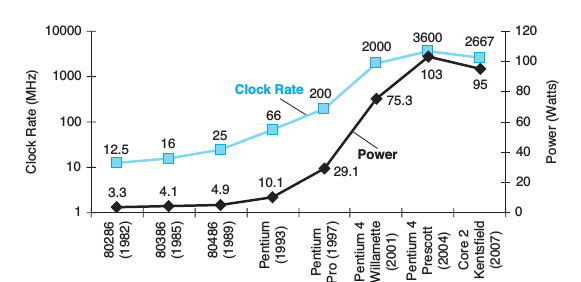
\includegraphics[width=0.8\textwidth]{images/cpu_clocks.png}
  \caption[Power wall]{The growth in CPU clock rates for 8 generations of x86 Intel processors and associated power consumption. By reducing input voltages to the processors
  engineers were able to keep power requirements low while increasing clock frequencies throughout the 1980s and 1990s. Limitations in semiconductor technology has, however,
  limited further increases in clock cycle rate. Taken from Patterson and Hennessy \cite[ch. 1]{patterson2009computer}.}
  \label{fig_clocks}
 \end{mdframed}
\end{figure}

\begin{figure}[ht!]
 \begin{mdframed}
  \centering
  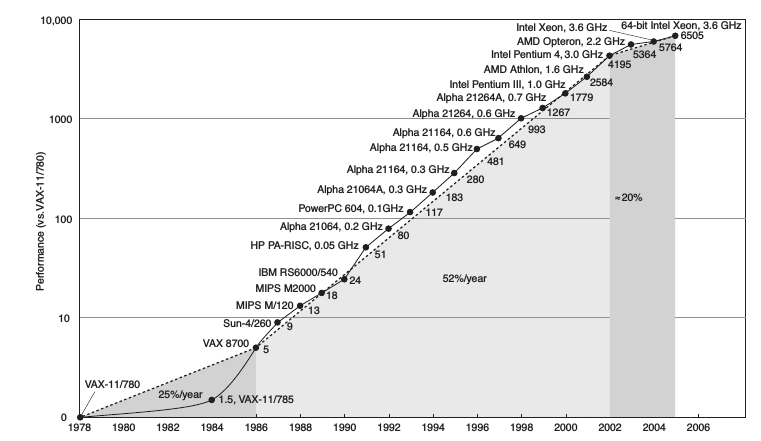
\includegraphics[width=0.8\textwidth]{images/runtime_decrease_cpu.png}
  \caption[Program response time decline]{Here processor performance is plotted relative to the VAX-11/780 measured by the SPECint benchmarks. The substantial growth seen after the mid-1980s
  are primarily due to increasingly advanced processor architectures. Since 2002 the growth has been slowed to below 25\% primarily due to the power wall and high memory latencies. Taken from Patterson and Hennessy \cite[ch. 1]{patterson2009computer}.}
  \label{fig_runtime_decrease_cpu}
 \end{mdframed}
\end{figure}

Since the latter half of the 2000s most desktop processors started subscribing to the Multiple Instruction Multiple Data (MIMD) paradigm where several processes 
(or \textit{threads}\footnote{Here a thread of execution is taken to be the basic unit of execution, with its own program counter and stack space, but sharing the address space with other threads started by the same process} of execution 
within a single process) is executed simultaneously within multiple \textit{microprocessors} on the same processor die (also known as processing cores). 
See Figure~\ref{fig_amd_barcelona_arch} for an example of such a multi-core layout. Modern processors is thus geared towards attaining higher throughput by better exploiting the 
abundance of task-level parallelism in modern day computer usage, instead of increasing the response rate of individual processes. Whereas once only a select number of compute 
programs warranted nodes with multiple processors (physical chips) per compute node, today any desktop software has to be able to use multiple compute streams (``threads'') 
in order to fully exploit the compute capacity of modern hardware \cite{patterson2009computer} \cite{akhter2006multi}. 
\begin{figure}[ht!]
 \begin{mdframed}
  \centering
  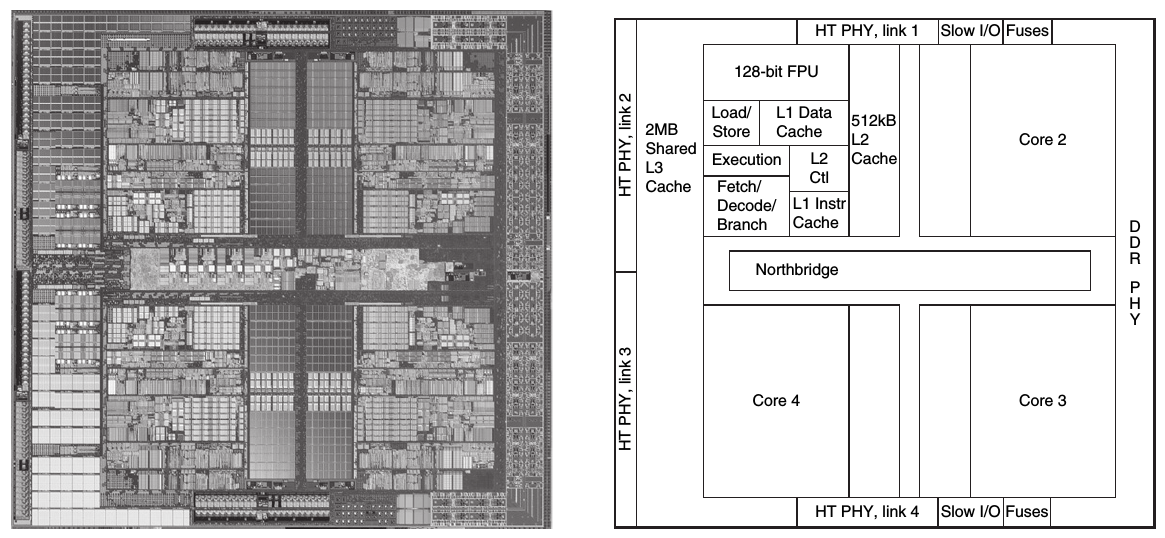
\includegraphics[width=0.8\textwidth]{images/amd_barcelona.png}
  \caption[AMD Barcelona]{Microphotograph and layout of the quad-core AMD Barcelona generation processor. Taken from Patterson and Hennessy \cite[ch. 1]{patterson2009computer}.}
  \label{fig_amd_barcelona_arch}
 \end{mdframed}
\end{figure}

\subsection{Fine- and course-grained hardware parallelism}
Due to the shift towards the MIMD paradigm most modern processors have both fine- and course-grained hardware parallelism. Well before the advent of multi-core processors instruction-level parallelism
existed. The original Pentium processor was able to pipeline instructions so that more than one instruction could be executed in a single clock cycle, by having 2 execution units. Keeping the execution units
busy most of the time has since become one of the key focuses of pipeline architectures. As such instructions without dependencies between them are no longer executed in parallel (starting with Pentium 
Pro processor [1995]). Later processors, such as the Pentium 4 (2002), has multiple units dealing with interrupt logic and processor state and is able to execute 2 logical threads concurrently per 
processor (and later processor core). This is known as \textit{simultaneous multithreading} \cite{gerber2002software,akhter2006multi}. See Figure~\ref{fig_cpu_arch_skylake} for an overview of the latest 
Intel Skylake generation microarchitecture.
\begin{figure}[ht!]
 \begin{mdframed}
  \centering
  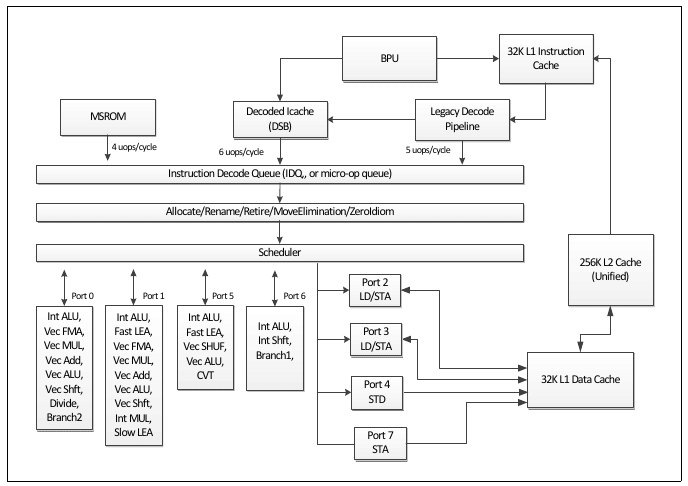
\includegraphics[width=0.8\textwidth]{images/cpu_intel_skylake.png}
  \caption[Intel Skylake Generation Architecture]{Architecture of the $6^\text{th}$ generation (Skylake) Intel Core processors (2015). As with many modern processors the front-end instruction fetch and decode components (apart from 
  the branch prediction unit) and back-end instruction retire components are all in-order components. Each logical core has access to an out-of-order execution engine with many arthmetic units in order to pipeline, issue and 
  execute multiple independent instructions simultaneously at hardware-level. Like most modern AMD and Intel processors each core has access to a level 1 cache to store instructions and data, as well as a larger L2 
  cache (32KB and 256 KB respectively for Skylake processors). All of the cores share a large L3 cache (up to 2MB per core). Picture and specifications taken from the Intel Architecture Optimization Guide \cite{intelArch}}
  \label{fig_cpu_arch_skylake}
 \end{mdframed}
\end{figure}

The advanced multiple-issue out-of-order execution engines parallelizes instruction execution at a hardware level, hidden from the application programmer. However, the ALUs of modern CPUs also support short 
SIMD vector operations. Figure~\ref{fig_SIMD} illustrates a typical SIMD computation. These instructions extend the original x86 instruction set with vector equivalents for many common operations. Originally
the MMX instruction set allowed only integer arithmetic operations on packed byte, word and doubleword registers and added eight additional 64-bit registers to the processor. Later extensions included 
various versions of Streaming SIMD Extensions (SSE) and Advanced Vector eXtensions (AVX), adding floating point and integer arithmetic on packed 128-bit and 256-bit registers respectively. These
SIMD vector operations improves the performance of tasks like 3D graphics and signal/image processing, that are inherently parallel, have localized recurring operations on data streams and have data-independent 
control flow. Most compilers (including the GNU compiler suite) vectorize code automatically when optimizations are enabled, but it may be necessary to write assembly code by hand in cases where the compiler fails
to do so (deeply nested loops is one such situation) \cite{intelArch}.
\begin{figure}[ht!]
 \begin{mdframed}
 \centering
  \begin{tikzpicture}[node distance=2.0cm,  
    block/.style={
      draw,
      fill=white,
      rectangle, 
      text width=2.0cm,
      inner sep=0.2cm}]
    \node (x4) [block] {x4};
    \node (x3) [block, right of=x4] {x3};
    \node (x2) [block, right of=x3] {x2};
    \node (x1) [block, right of=x2] {x1};
    \node (y4) [block, below of=x4] {y4};
    \node (y3) [block, below of=x3] {y3};
    \node (y2) [block, below of=x2] {y2};
    \node (y1) [block, below of=x1] {y1};
    \node (o4) [below of=y4]{$\oplus$};
    \node (o3) [below of=y3]{$\oplus$};
    \node (o2) [below of=y2]{$\oplus$};
    \node (o1) [below of=y1]{$\oplus$};
    \node (r4) [block, below of=o4] {x4$\oplus$y4};
    \node (r3) [block, below of=o3] {x3$\oplus$y3};
    \node (r2) [block, below of=o2] {x2$\oplus$y2};
    \node (r1) [block, below of=o1] {x1$\oplus$y1};
    \draw [rarrow] ($(y4) - (0.5,0)$) -- (o4);
    \draw [rarrow] ($(y3) - (0.5,0)$) -- (o3);
    \draw [rarrow] ($(y2) - (0.5,0)$) -- (o2);
    \draw [rarrow] ($(y1) - (0.5,0)$) -- (o1);
    \draw [rarrow] (x4) -- (o4);
    \draw [rarrow] (x3) -- (o3);
    \draw [rarrow] (x2) -- (o2);
    \draw [rarrow] (x1) -- (o1);
    \draw [rarrow] (o4) -- (r4);
    \draw [rarrow] (o3) -- (r3);
    \draw [rarrow] (o2) -- (r2);
    \draw [rarrow] (o1) -- (r1);
  \end{tikzpicture}
 \caption[Vector operation]{A typical Single Instruction Multiple Data (SIMD) vector operation. Here $\oplus$ is any binary arithmetic or logical operator. Some variants on this instruction layout exist, but they all perform the same operation
			    on multiple data elements packed into extended registers}
 \label{fig_SIMD}
 \end{mdframed}
\end{figure}

Both instruction-level parallelism and SIMD vector operations are fine-grained parallel processes handled by hardware. Since most modern processors have multiple processing cores operating systems can not only achieve concurrent thread execution 
(where the execution of multiple threads are interleaved on physical hardware), but truly parallel execution of threads on multiple processor cores. One threading API that has found widespread cross-platform use is the OpenMP standard \cite{openmp}, which is currently
implemented by the major Fortran, C and C++ compilers, including the Microsoft C++, Intel and GNU compiler suites. OpenMP provide parallelization options for both task- and data-parallel problems, is based on the lightweight fork-join threading pattern and
takes care of thread instantiation and termination automatically. Most sections and loops can therefore be parallelized by simply specifying a single compiler directive in front of the block of code to be parallelized. OpenMP also support static and dynamic
scheduling options that are useful in problems that require load-balancing to perform well \cite{openmp,akhter2006multi}.
\section{Many-core GPU architectures}
Much of the discussion in this chapter is drawn from Kirk and Hwu \cite[ch. 1-3]{kirk2012programming}, Owens et al. \cite{owens2008gpu} and the Compute Uniform Device Architecture (CUDA)
programming reference \cite{cuda}. Our discussion is focused towards implementation in NVIDIA CUDA. We start by giving the reader an historical overview and then highlight the key differences
in architecture that set GPUs appart from CPUs.
\subsection{Historical development}
Today's modern programmable GPU devices have evolved from the fixed-pipeline graphics hardware of the 1980's and 1990's. Driven by the demand
for high resolution graphics in the video game industry modern devices must be able to render billions of pixels per second (72 giga pixels per second 
for the latest Maxwell GTX980 devices \cite{gtx980}). From inception these devices favored achieving high throughput over higher operational latencies compared to traditional
CPU-based computing. The steps involved with transforming primitives (typically triangles) in world space to rasterized images rendered by a display takes thousands
of compute cycles from start to finish. However the coordinate, lighting and per-pixel shading operations are data-parallel operations. In addition the stages within
the graphics pipeline can be computed in parallel; while new primitives enter the pipeline the rasterization and fragment processing of primatives previously transformed is 
completed, enabling both data- and task-parallelism on GPUs. The major steps in the graphics pipeline is shown in Figure~\ref{fig_graphics_pipeline} for reference.

\begin{figure}[ht!]
 \begin{mdframed}
 \centering
  \begin{tikzpicture}[node distance=2.8cm,  
    block/.style={
      draw,
      fill=white,
      rectangle, 
      text width=2.0cm,
      inner sep=0.2cm}]
    \node (app) [block] {3D application / game};
    \node (api) [block, right of=app] {3D API \& drivers};
    \node (fe) [block, below of=app] {GPU front end};
    \node (assembly) [block, right of=fe] {Primitive assembly};
    \node (rasterization) [block, right of=assembly] {Rasterization and interpolation};
    \node (rasterops) [block, right of=rasterization] {Raster operations};
    \node (fb) [block, right of=rasterops] {Framebuffer};
    \draw [dashed,transform canvas={yshift=-1.4cm}] ($(app) - (0.5cm,0)$) -- (fb |- app) node [right, above] (cpu) {CPU} node [right, below] (gpu) {GPU};
    \draw [rarrow] (app) -- (api);
    \draw [rarrow] (api) -- (fe);
    \draw [rarrow] (fe) -- (assembly);
    \draw [rarrow] (assembly) -- (rasterization);
    \draw [rarrow] (rasterization) -- (rasterops);
    \draw [rarrow] (rasterops) -- (fb);
  \end{tikzpicture}
 \caption[Graphics pipeline]{The classical graphics pipeline. At the front end of the pipeline verticies are transformed, colours assigned,
 texture coordinates and normals calculated. The rasterization step interpolate per-primitive data, such as colour, across all the pixels 
 touched by the triangle formed between vertex triples. Raster operations performs final blending and anti-aliasing operations, before the images written
 out to the display frame buffer.}
 \label{fig_graphics_pipeline}
 \end{mdframed}
\end{figure}

The requirement of transforming, rasterizing and shading possibly millions of triangle primitives driving GPU development clearly diverges from the requirements behind the
design of traditional CPUs. CPU development is driven by the need to process large sequential programs per CPU core, each containing complex branching and diverse memory access patterns, 
whereas GPUs are driven by the need to apply the same set of basic operations to many elements (or ``Single Instruction Multiple Data'' [SIMD]) paradigm that graphics processing subscribes to. 
Whereas CPUs use several tiers of large caches to hide the latencies of memory accesses GPUs have relatively little on-chip cache memory per basic compute (``Streaming Processor'' [SP]) 
unit. Instead of caching GPUs rely mostly on the amount of parallel work available to each SP unit and a fast context switching / work scheduling mechanism to ensure each of the SPs are 
occupied with work while memory transactions are completed for threads stalled by load and store operations.

Although the hardware platform could potentially be employed for applications other than 3D graphics it wasn't until the early 2000's that programmable graphics hardware became widely
available. For instance the NVIDIA GeForce 3 exposed the internal instruction set of the vertex processor to the application developer. Soon the ATI Radeon 9700 and GeForce FX 
made the fragment shading process, normally part of the rasterization and interpolation step, reprogrammable. At this point the vertex and fragment shading units were run on separate
hardware. The XBox 360 (2005) introduced an early unified vertex and fragment shader processor.

Even though the hardware now supported extending the traditional graphics pipeline to do more complex operations it was still impractical to use the highly parallel hardware for 
computational processes other than small research projects. Computational problems had to be mapped to the standard graphics operands: verticies and textures. Other problems
such as the lack of scattered memory writes limited the applicability of the platform to a small number of problems.

This was addressed by a series of software and hardware developments that aimed to to give application developers access to the processors without having to call
on Graphics APIs. Of those developments BrookGPU \cite{buck2004brook} was an early abstraction away from graphics primatives. It recasted computation in terms of small programs (``kernels'') operating
on ``streams'' of input data elements (arrays of values that can be operated on in parallel). This paradigm sets GPUs aside from ordinary vector processors that loads a series of values from global
memory, performs a simple mathematical operation on each of the elements and write the results back to global memory. Instead stream processors can load values from local register memory, performing multiple
operations on each of these values before storing the results (possibly to local memory). The paradigm allows for achieving greater arithmetic intensity (a single memory operation is followed
by many computations) and is critical for hiding the high latencies of memory accesses experienced on GPUs. 

More recently NVIDIA CUDA \cite{cuda} and the OpenCL standard \cite{opencl} have become widely used in programming GPUs to perform general scientific computing in a variety of fields including the signal 
processing domain. Both lend themselves to the streaming processor paradigm and facilitate the implementation
of the following generally-used parallel computing primitives:
\begin{itemize}
 \item Scatter/gather: The addresses used in memory accesses (both load and store) can be computed.
 \item Map: an operation is applied to every element in the stream. Typically many threads will be launched
       each reading an element from the stream, performing the operation on that element and writing the value
       back to memory afterwards.
 \item Reduce: By applying a binary associative operation repeatedly, an array of values is reduced to a single value.
       An example is ordinary summation, minimums/maximums, variance, etc. These operations typically split the data up into
       subsets, performing many additions in parallel and repeating the process on the set of results until a single value is
       obtained. 
 \item Scans: Scan and prefix scan operations are widely used in parallel programming (for instance index calculations, as used
       in our work). A scan of an array contains the running accumulations (in the case of summation) of elements in an array. 
\end{itemize}

\subsection{Modern programmable GPU architecture}
The difference in design philosophy is reflected in the substantial differences in the architectures of modern GPUs and CPUs. CPUs dedicate a significant portion die area to large caches and complex control logic dealing with
branch prediction and scheduling. GPUs on the other hand dedicate a significant portion of die area to arithmetic and other execution units and rely on having enough arithmetic work to occupy most of those units most of the time.
Figure~\ref{fig_cpu_gpu_diff} illustrates the proportions of both CPU and GPU die area spent on arithmetic.
\begin{figure}[ht!]
 \begin{mdframed}
  \centering
  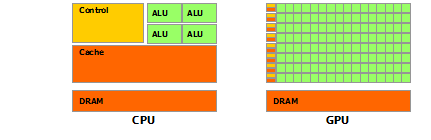
\includegraphics[width=0.5\textwidth]{images/gpu-devotes-more-transistors-to-data-processing.png}
  \caption[CPU vs. GPU architecture]{The proportion of transistors allocated to arithmetic processing in CPUs and GPUs. Taken from the NVIDIA programming reference \cite{cuda}}
  \label{fig_cpu_gpu_diff}
 \end{mdframed}
\end{figure}

Modern GPUs works best in problem contexts where a significant portion of the computation is data-parallel. In CUDA nomenclature (similar concepts exist in OpenCL) the parallel work is broken up into a \textit{grid} of
separate thread \textit{blocks} (see Figure~\ref{fig_grid_blocks} for an illustration). In each of these blocks on-chip memory resources is shared, limiting the size of the individual blocks. On current NVIDIA GPUs there is a hard limit (1024) for the number of 
threads within a block, however the amount of special memory (including register memory) available to each of these blocks may further limit the number threads in the block that can physically execute simultaneously. Using streaming processor terminology 
each of the blocks would therefore process a portion of stream memory. Blocks are in turn subdivided into \textit{warps} of threads (currently 32 threads form a warp) that execute instructions in lockstep. This means that when one
thread inside a warp is stalled (for instance a memory access or a synchronization barrier) the entire warp is stalled. Unlike the instruction scheduling system of CPUs the schedulers in GPUs don't contain complex branch prediction logic; when some
threads in a warp require the execution of one of the directions in a branch while the rest take another direction both sides of the branch is evaluated and the results are simply masked out for those threads that are unaffected
by the branch direction. The requirement of lockstep execution places a hefty penalty on branch divergence within the instruction kernels, as well as memory accesses that don't adhere to the alignment specifications of the GPU. Note that this description of how work 
is specified out in a high level programming language is independent of specifics of the device the work is to be processed on. The individual blocks can be mapped onto the targeted device 
in any order and in any quantity, depending on the resources of the device. Each block of work should therefore perform its computation in isolation of the remaining blocks. Although 
intra-block communication between threads and synchronization is possible, inter-block communication is only possible through accesses to off-chip memory and should be avoided.
\begin{figure}[ht!]
 \begin{mdframed}
  \centering
  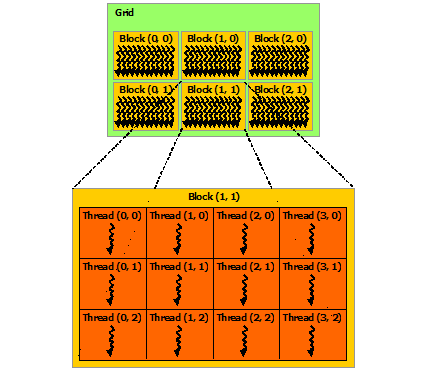
\includegraphics[width=0.45\textwidth]{images/grid-of-thread-blocks.png}
  \caption[Thread layout in CUDA]{The layout of work threads in CUDA. Taken from the NVIDIA programming reference \cite{cuda}}
  \label{fig_grid_blocks}
 \end{mdframed}
\end{figure}

At a hardware level GPUs comprise of multiple \textit{Streaming Multiprocessors}, each containing many \textit{Stream Processors} capable of performing arithmetic operations (predominantly IEEE 754 single precisision floating point) along
with several special function units, warp-schedulers and memory load/store units. Figure~\ref{fig_kepler_arch} shows the layout of Kepler-generation NVIDIA GPUs. The exact number of Streaming Multiprocessors and Stream Processors
vary between generations of GPUs, but the total number of Stream Processors per GPU tend to double every 2 years. Depending on the resource constraints of each of the thread blocks several blocks may be mapped to a single 
Streaming Multiprocessor for simultaneous execution. The warp schedulers schedule warps that have instructions (along with the required operand data) ready for execution onto sets of Stream Processors, dispatching multiple independent 
instructions onto individual Stream Processors per clock cycle (depending on the number of dispatch units available per Multiprocessor). Warps that are stalled (for example waiting on a load/store operation) is switched out of context
and replaced with warps that have operands ready for processing, thereby hiding memory access latencies. Ideal kernels should therefore:
\begin{itemize}
 \item Contain enough independent arithmetic instructions to occupy all the Stream Processors during
       any given clock cycle.
 \item Access to both on- and especially off-chip memory should be kept to a minimum and subscribe to coalesced access patterns, especially considering that the number of load/store units are far fewer than the number of
       single precision units and peak memory bandwidth is on the order of 60x lower (Kepler generation) than the peak single precision compute throughput of the device. In other words the arithmetic intensity should be high, as
       is the case in typical graphics shading operations for instance.
 \item There must be enough warps of work scheduled to the GPU to keep the Multiprocessors occupied most of the time.
 \item Special memory resources (including registers) should be used sparingly to ensure the Streaming Multiprocessor is not starved of resources as this lowers the number of warps that can be executed at any given point in time 
      (``effective occupancy'').
\end{itemize}
\begin{figure}[ht!]
 \begin{mdframed}
  \centering
  \begin{subfigure}[b]{0.7\textwidth}
    \centering
    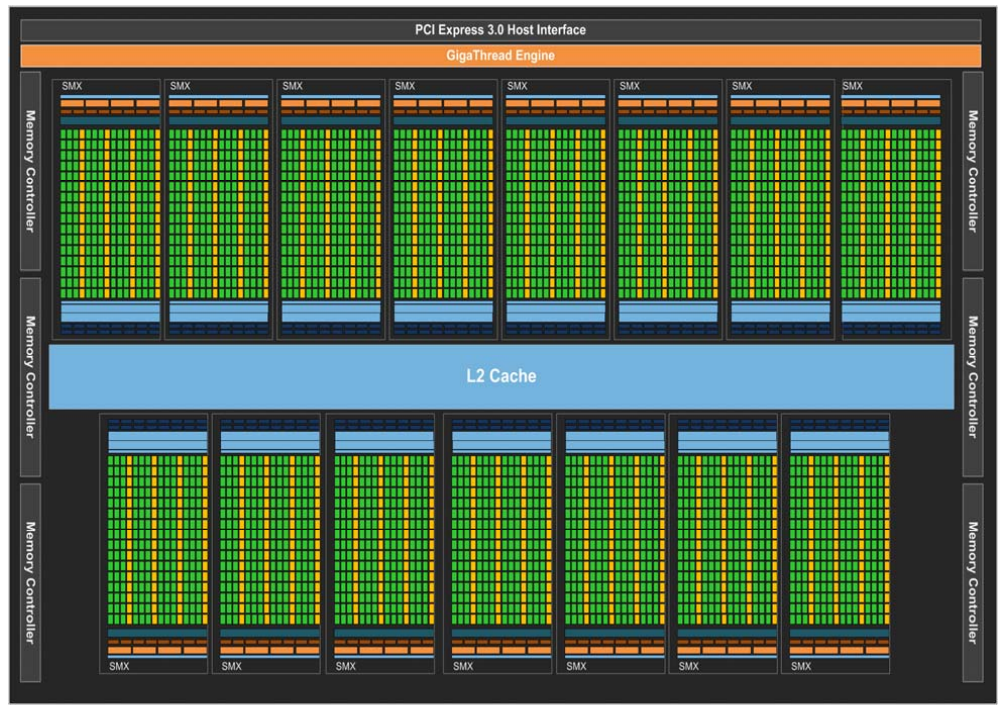
\includegraphics[width=\textwidth]{images/kepler_arch.png}
    \caption{}
  \end{subfigure}
  \begin{subfigure}[b]{0.6\textwidth}
    \centering
    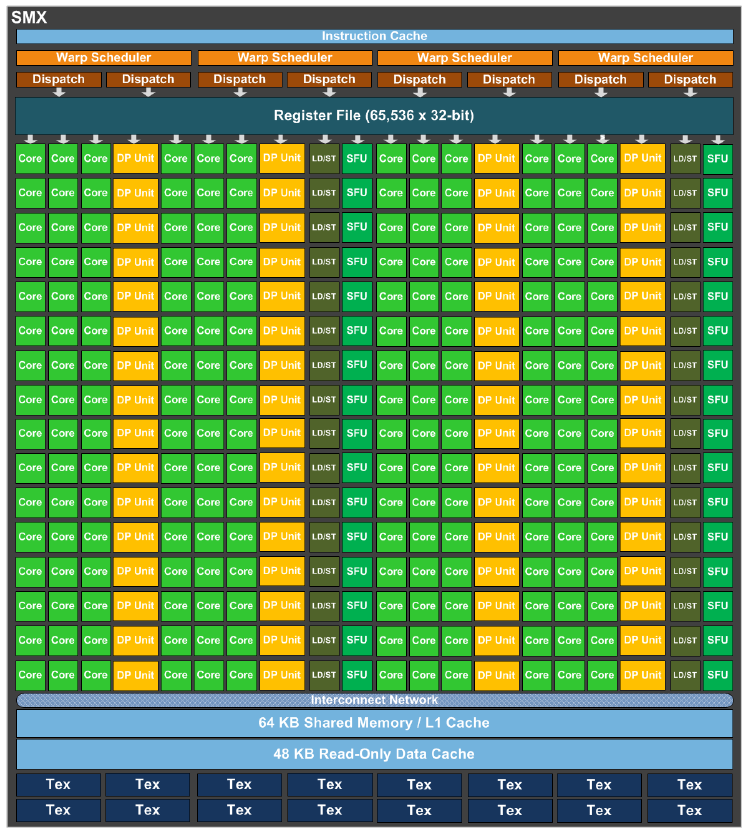
\includegraphics[width=\textwidth]{images/kepler_smx_arch.png}
    \caption{}
  \end{subfigure}
  \caption[Kepler architecture]{Kepler die architecture. (a) shows the overall die layout, containing 15 Streaming Multiprocessors. (b) shows the layout of each multiprocessor, containing one double precision unit for every 
				3 single precision units, 1 load/store and 1 special function unit for every 6 single precision units. The total number of registers, local and shared memory is split between the number of threads per 
				block, determining how many blocks can be executed simultaneously. Taken from the Kepler whitepaper \cite{kepler}}
  \label{fig_kepler_arch}
 \end{mdframed}
\end{figure}

\subsection{GPU memory layout}
The GPU memory hirarchy is substantially different from those found on CPUs. As we pointed out earlier the total cache memory
per Multiprocessor is divided between many Stream Processors. The following special memory systems exist on the GPU:
\begin{itemize}
 \item Shared instruction cache. GPUs are SIMD devices by nature and thus require the same set of instructions to be executed
 by many Stream Processors. This means that the instruction cache can be shared between many Stream Processors, unlike with CPUs
 where each core has its own instruction cache.
 \item Local memory: Each Stream Processor has access to its own private local memory space in which register memory reside. The total number of
 registers is divided amongst all threads and is determined by the maximum number of registers needed to execute the instructions contained in a 
 kernel, setting the upper limit to how many threads can be executed on the Multiprocessor at any point in time. 
 \item L1 data cache: The L1 cache on GPUs is split into a local data cache and a shared memory cache. On GPUs the local cache stores register 
 spills from local memory. Depending on the hardware generation L1 memory also caches accesses to global memory (2.x by default), but this is
 not necessarily done by all devices. Some 3.x Kepler devices can opt in to this behavior by specifying compile time options.
 \item Shared memory: As suggested shared memory is a cache memory shared between all threads executing in a block. The split of the L1 cache into
 shared and data caches is reconfigurable at run-time. It is also important to note that the exact amount of shared memory requested by each kernel at 
 launch sets the limit on how many blocks of that kernel can be executed simultaneously. Shared memory is used for both communication between threads as well
 as storing values that are commonly accessed (and/or modified) by multiple threads. Importantly for performance, however, it is worth mentioning that
 shared memory is divided in banks; each consecutive word falls into a different bank. An out-of-sequential-order or strided reads between two or more threads
 can result in accesses to the same bank simultaneously, generating a bank conflict. Special rules apply for sub-word and multiple-word accesses, for
 which the reader can refer to the CUDA API \cite[Section G: Compute Capabilities]{cuda}.
 \item Constant cache: Constant memory is read-only memory that resides in off-chip memory, but is cached on chip. CUDA uses this mechanism to broadcast
 a single read to a half-warp of threads thereby saving 15/16 memory accesses that would be encountered when the same read pattern is made to global memory without 
 this mechanism. Consecutive accesses to the same memory encounters no extra cost.
 \item Read-only data (texture) cache: In graphics processing one of the most common operations performed by the GPU is to map textures onto triangle primitives. 
 Memory reads to textures (stored off-chip) is highly regular and spatially coherent, meaning that a group of work units will likely read values from the same area of texture
 memory. The caching mechanism is designed to optimize this access pattern. The texture cache residing in each Multiprocessor is not kept up to date with changes made to
 textures in global memory and can become stale. Loads from texture memory can also be made with hardware-based interpolation between neighboring values enabled.
 \item Global memory: Global memory resides off chip, just like constant and texture memory. Global memory accesses are cached in the crossbar L2 cache that 
 is shared between Multiprocessors and has a cache-line length of 32-bytes. In Fermi accesses were further cached in the L1
 data cache by default, where the cache lines were 128 bytes in length. With some compute 3.x hardware this caching option can be enabled. Some read-only 
 accesses are cached in the read-only data cache in compute 3.x devices. Warp memory accesses (not essentially ordered on an intra-warp level) that are aligned 
 with these boundaries maximizes available memory bandwidth.
\end{itemize}
